% ----------------------------------------------------------------------
% Template VERIFICA
% ----------------------------------------------------------------------
% 2020 di d!egofantinelli at jazzmagus@gmail.com
% ----------------------------------------------------------------------

% ---------------------------------- Preambolo
\documentclass[11pt, a4paper]{exam}
\usepackage[T1]{fontenc}
\usepackage{mdframed}
%\usepackage{nicefrac}
%\usepackage[applemac]{inputenc}
%\usepackage[utf8]{inputenc}
\usepackage[italian]{babel}
\usepackage[margin=1.3in]{geometry}
\usepackage{amsmath,amssymb}
\usepackage{multicol}
\usepackage{graphicx}
\usepackage{tikz}
\usepackage{upquote}
\usepackage{caption}
%\usepackage{fancyhdr}
\usepackage{float}

\printanswers

% ---------------------------------- Command
\renewcommand{\questionshook}{%
    \setlength{\leftmargin}{0pt}%
}
\renewcommand{\choiceshook}{%
    \setlength{\leftmargin}{20pt}%
}

\newcommand{\class}{\huge {Verifica di Matematica}}
\newcommand{\term}{Recupero Primo Quadrimestre}
%\newcommand{\examnum}{Verifica numero: 1}
\newcommand{\examdate}{03 marzo 2021}
\newcommand{\timelimit}{50 minuti}

\CorrectChoiceEmphasis{\color{red}}
\SolutionEmphasis{\color{red} \footnotesize}
\renewcommand{\solutiontitle}{\noindent\textbf{Soluzione:}\par\noindent}

% ---------------------------------- Headers and Footers

\pagestyle{headandfoot}
\firstpageheader{IIS "G. A. Remondini" - Bassano del Grappa (VI)}{}{\examdate}
\runningheader{\footnotesize VERIFICA di Recupero di MATEMATICA}{}{Classe 5\string^QA}
\runningheadrule

\firstpagefooter{}{}{pag. \thepage\ di \numpages}
\runningfooter{}{}{pag. \thepage\ di \numpages}
\runningfootrule

% ---------------------------------- Punteggi
\pointpoints{punto}{\em punti}
\pointformat{[{\footnotesize \thepoints}]}
\bonuspointpoints{punto bonus}{\em punti bonus}
\bonuspointformat{[{\footnotesize \thepoints}]}
\pointsinrightmargin
\setlength{\rightpointsmargin}{.2cm}
\chqword{Esercizio}
\chpword{Punti}
\chbpword{Punti Bonus}
\chsword{Punteggio}
\chtword{Totale}

\begin{document}

% ---------------------------------- Title Page
\begin{center}
\rule[2ex]{\textwidth}{0.5pt}\\
{\huge{\bf \class}}\\[12pt]
%{\huge -\, \term \, - }\\[8pt]
\rule[2ex]{\textwidth}{0.5pt}\\
\end{center}
\vspace{3cm}
\begin{tabular*}{\textwidth}{l @{\extracolsep{\fill}} r @{\extracolsep{6pt}} l}
\textbf{} & \textbf{Nome e Cognome:} & \makebox[2.5in]{\hrulefill}\\
\textbf{} &&\\
\textbf{} & \textbf{Classe:} & \makebox[2.5in]{\Large{\bf 5 \string^ QA}}\\
\textbf{} &&\\
\textbf{} & Tempo a disposizione: & \makebox[2.5in]{\timelimit}
\end{tabular*}\\[3cm]
\vspace{5cm}
% ---------------------------------- Avvertenze

\noindent
%\rule[2ex]{\textwidth}{0.2pt}
\textbf{Avvertenze}:
\begin{itemize}
	\item La presente Verifica - che viene somministrata in modalit� DDI - contiene \numquestions \; quesiti, per un totale di \numpoints \;punti.
	\item La webcam dovr� rimanere accesa per tutto il tempo della verifica (\timelimit), salvo impossibilit� concrete di connessione; il microfono rester� spento e verr� acceso soltanto per chiarimenti e domande, che saranno consentite negli ultimi 20 min della prova.
	\item E' vietato l'utilizzo di calcolatrici scientifiche, smartphone, tablet e altri dispositivi digitali, nonch� la consultazione di testi, appunti e siti web.

\end{itemize}%\rule[2ex]{\textwidth}{0.2pt}
\vfill
\newpage

% ---------------------------------- Esercizio 1

\begin{questions}

\addpoints
\question
Determinare l'Insieme di Definizione delle seguenti Funzioni \(f : x \in \mathbb{R} \to  y \in \mathbb{R}\):\\
\begin{parts}
\part[5]
\( y= {\sqrt{\dfrac{1}{1+5x-6x^2}}}\)\\
%\fillwithlines{0.5in}
{\footnotesize
\begin{solution}
	\(D=\{x \in \mathbb{R} : -\dfrac{1}{6} < x < 1\}\)
\end{solution}
}
\vspace{.5cm}

\part[5]
\( y = \sqrt{5 - x} + \sqrt{x^2 - 4}\)\\
%\fillwithlines{0.5in}
{\footnotesize
\begin{solution}
	\(D = \{x \in \mathbb{R} : x \le -2  \lor 2 \le x \le 5\}\)
\end{solution}
}
\vspace{.5cm}

\part[5]
\( y= f(x) = {\dfrac{1}{x^3 - 25x}}\)\\
%\fillwithlines{0.5in}
{\footnotesize
\begin{solution}
	\(D = \{x \in \mathbb{R} : x \neq 0 \, \land x \neq \pm 5\}\)
\end{solution}
}

\end{parts}
\vspace{.8cm}

%------------------------------------------- Esercizio 2
\addpoints
\question [8] Per la seguente funzione: \[y= f(x) = {\sqrt{\dfrac{x^2 + 2}{x^2 - 1}}}\]

determina:

\begin{itemize}
	\item Insieme di Definizione;
	\item Intersezione con gli assi di simmetria;
	\item Segno della Funzione;
	\item Rappresenta graficamente i risultati.
\end{itemize}

%\fillwithlines{1in}
{\footnotesize
\begin{solution}
	\(D = \{x \in \mathbb{R} : - \infty < x < - 1 \land 1 < x < +\infty\}\)\\intersezioni: n� con asse $x$ n� con asse $y$;\\
	Studio del Segno: \( f(x) \ge 0 \quad \forall x \in D\) \end{solution}
}
\begin{figure}[H]
\flushleft
	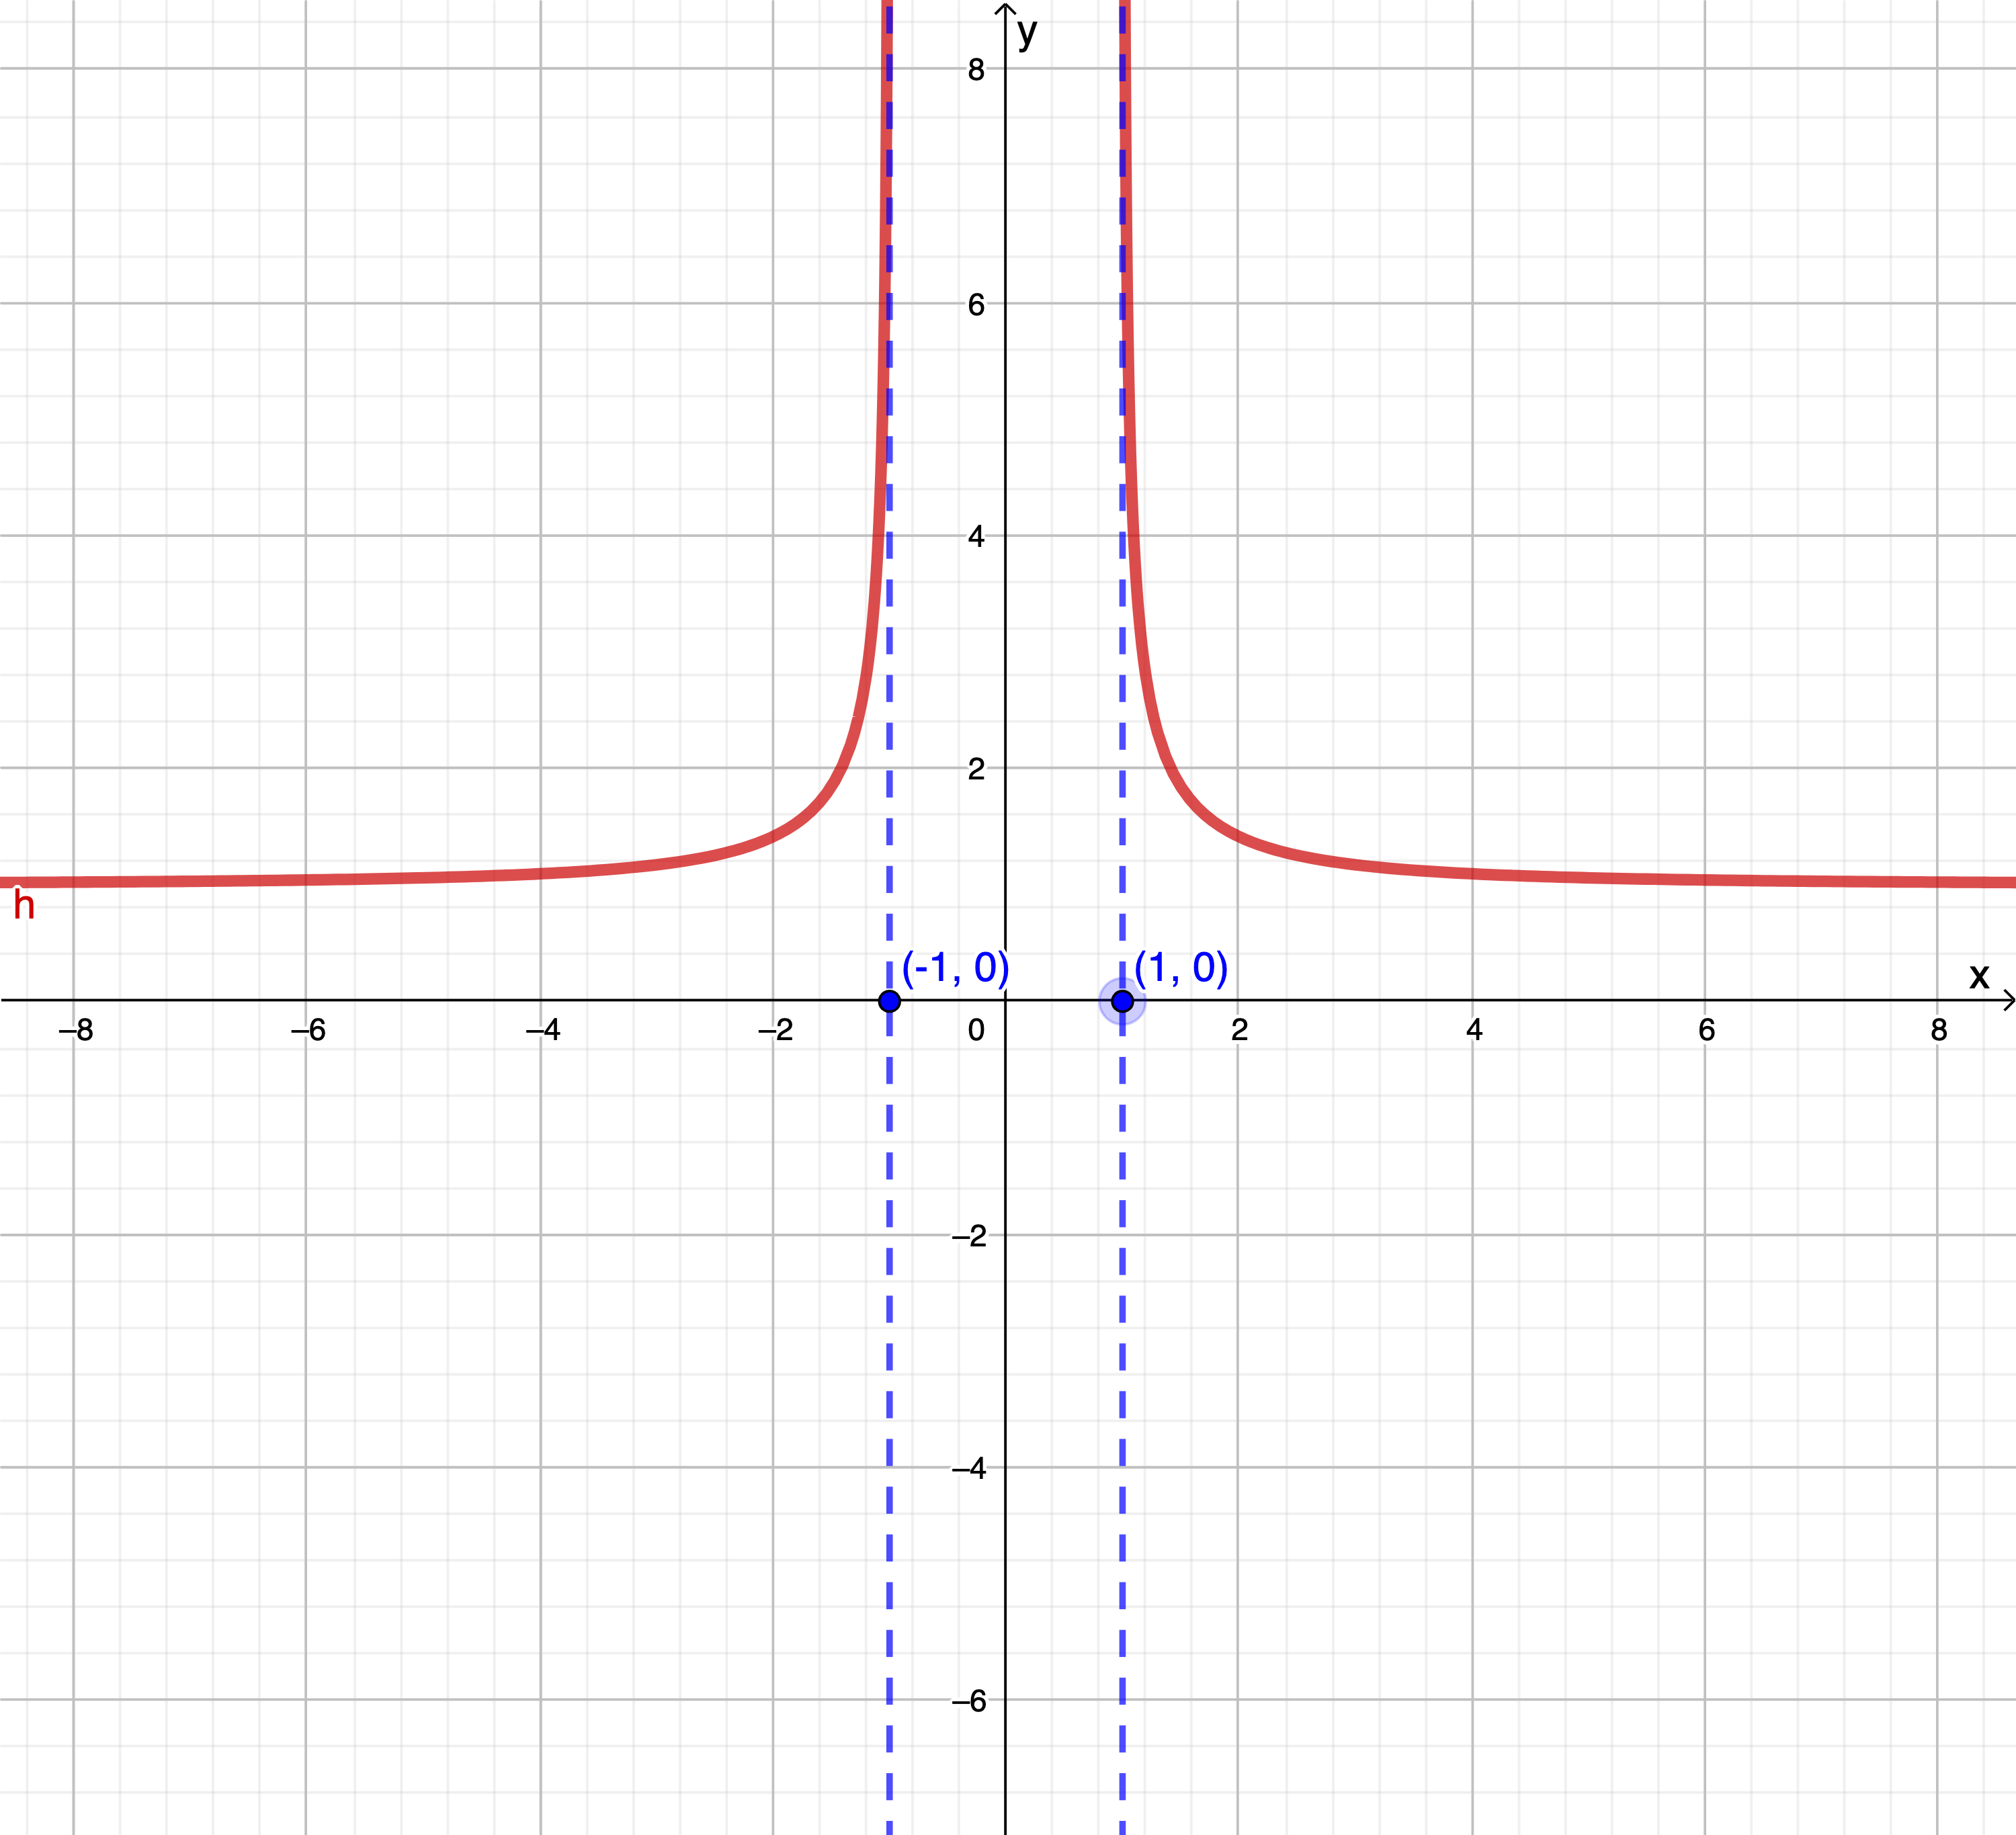
\includegraphics[width=\textwidth]{graph_01}
	\caption{Grafico ipotetico della funzione \(y= f(x) = {\sqrt{\dfrac{x^2 + 2}{x^2 - 1}}}\)}
    \label{fig:mesh1}
\end{figure}

\pagebreak
%------------------------------------------- Esercizio 3

\addpoints
\question [7] Quello riportato in figura � il grafico di una certa {\em Funzione Razionale Fratta}; determina:
\begin{itemize}
	\item Insieme di Definizione;
	\item Intersezione con gli assi di simmetria;
	\item Segno della Funzione;
\end{itemize}

%\fillwithlines{1in}
\begin{figure}[H]
	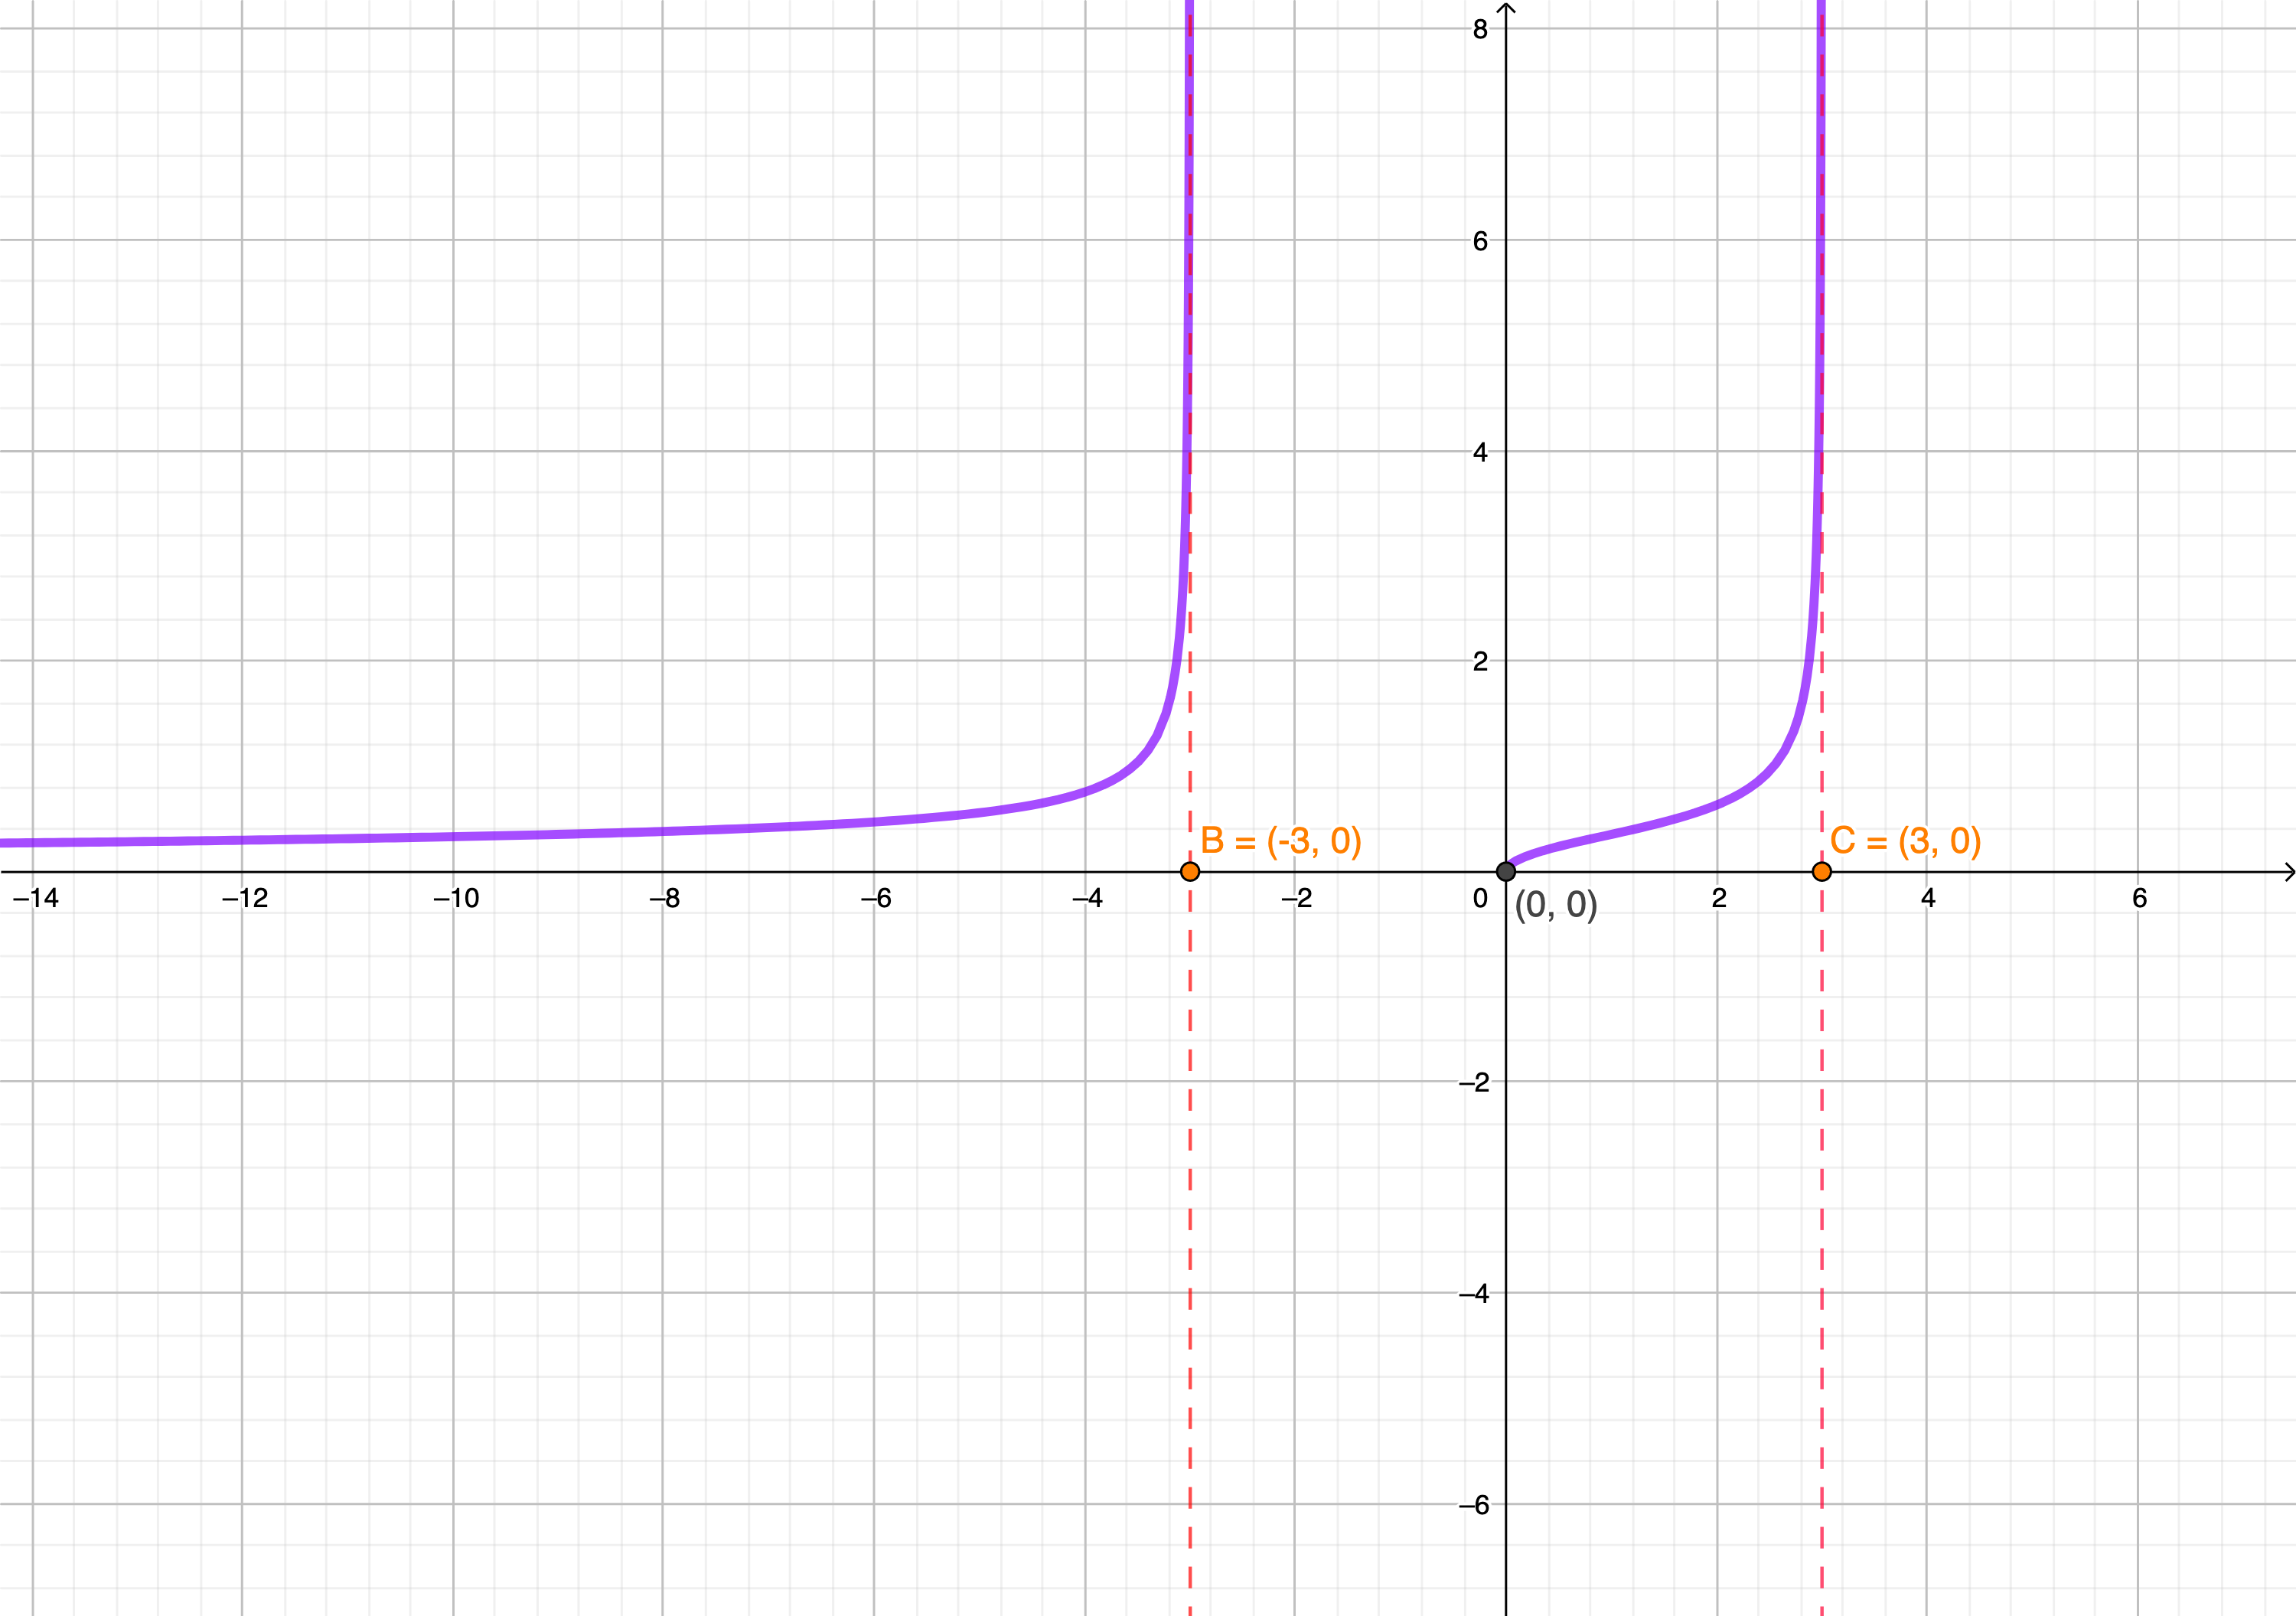
\includegraphics[width=\textwidth]{fun_irr_frac}
	\caption{Grafico di una funzione {\em Irrazionale Fratta}}
    \label{fig:mesh1}
\end{figure}
\end{questions}

\vfill

\noindent
\rule[2ex]{\textwidth}{1pt}
\begin{center}
{\bf Tabella dei punteggi}

\vspace{10pt}
\combinedgradetable[v][questions]
\end{center}
\vspace{8pt}
\footnotesize La sufficienza � fissata a 18 punti, ma potr� subire delle modifiche in fase di correzione, al fine di garantire la validit� della prova anche nel caso in cui si riscontrassero prestazioni della classe sensibilmente lontane dalla media-classe stimata.

\end{document}
